% This version of CVPR template is provided by Ming-Ming Cheng.
% Please leave an issue if you found a bug:
% https://github.com/MCG-NKU/CVPR_Template.

\documentclass[review]{cvpr}
%\documentclass[final]{cvpr}

\usepackage{times}
\usepackage{epsfig}
\usepackage{graphicx}
\usepackage{amsmath}
\usepackage{amssymb}

%\usepackage[ruled,noend,linesnumbered]{algorithm2e}
\usepackage{graphicx,color,psfrag}
\usepackage{amsfonts}
\usepackage{bigdelim}
\usepackage{dsfont}
\usepackage{color, soul}
\usepackage{graphicx}
\usepackage{caption}
\usepackage{subcaption}
\usepackage{cite}
\usepackage{dsfont}

% Include other packages here, before hyperref.

% If you comment hyperref and then uncomment it, you should delete
% egpaper.aux before re-running latex.  (Or just hit 'q' on the first latex
% run, let it finish, and you should be clear).
\usepackage[pagebackref=true,breaklinks=true,colorlinks,bookmarks=false]{hyperref}


\def\cvprPaperID{} % *** Enter the CVPR Paper ID here
\def\confYear{CVPR 2023}
%\setcounter{page}{4321} % For final version only


\begin{document}

%%%%%%%%% TITLE
\title{Hand-Object Pose Estimation from RGBD Images}

\author{First Author\\
Institution1\\
Institution1 address\\
{\tt\small firstauthor@i1.org}
% For a paper whose authors are all at the same institution,
% omit the following lines up until the closing ``}''.
% Additional authors and addresses can be added with ``\and'',
% just like the second author.
% To save space, use either the email address or home page, not both
\and
Second Author\\
Institution2\\
First line of institution2 address\\
{\tt\small secondauthor@i2.org}
}

\maketitle


%%%%%%%%% ABSTRACT
\begin{abstract}
Hand-object pose estimation aims to predict the pose and shape of both the hand and held object under interaction. Although numerous applications in the real world such as augmented and virtual reality, hand-object pose estimation concerns relatively less attention. Several methods separately estimate hand shapes and object poses but totally neglect the correlations between hands and objects. In this work, we introduce an approach that leverages the advantage of the voting mechanism to jointly learn the appearance of hands and objects from RGB-D images. We propose a module called adaptive fusion to effectively collaborate RGB and Depth features by adaptively adding the weight for each type of feature before fusing. The output features can discriminate the differently meaningful distribution between color and depth information at each position. Moreover, we embrace the graph convolutional network (GCN) to learn the interaction relationships between the hand and held object shapes under manipulation. Unlike conventional methods looking at the center points of the hand and objects, our approach takes into account the hand and object keypoints that belong to their surfaces to estimate the shapes and learn the correlations. This facilitates examining the geometric constraints and spatial restrictions to achieve accurate outcomes. Experiments using benchmark datasets illustrate that our network achieves beyond state-of-the-art accuracy in 3D pose estimation.
\end{abstract}

%%%%%%%%% BODY TEXT

%
\section{Introduction}
\label{sec:intro} 
Estimation of hands and objects is fundamental and crucial for understanding meaningful interpretation of human action and
behaviour. It provides enormous knowledge for environmental perception and teaching manipulating systems. With the advent of deep learning, pose estimation tasks have significantly made progress such as RGB-based \cite{cai20203d, zimmermann2017learning, gao2019variational, xiang2017posecnn, tremblay2018deep}, depth-based \cite{oberweger2017deepprior++, moon2018v2v, xiong2019a2j, ge20173d, cai2022ove6d, li2020category}, and RGB-D methods \cite{kazakos2018fusion, yuan20193d}. Jointly estimation of hands objects under interaction, however, has attracted less attention due to chronic challenges. This requires simultaneously predicting the pose and shape of hands and objects during the hands handling and executing the objects. In this paper, we propose a novel network to tackle this problem from RGB-D images. 

\begin{figure}[t]
\center
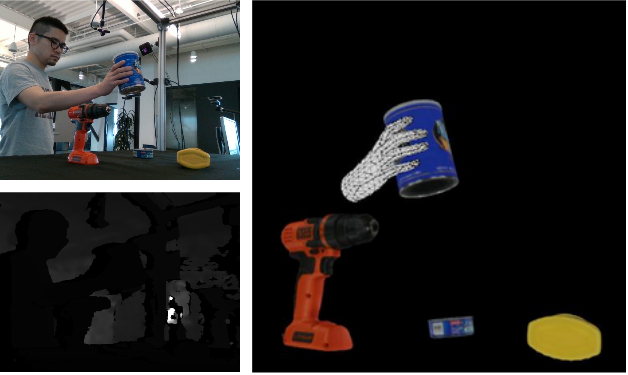
\includegraphics[width=\linewidth]{Figs/result_exp.png}
\label{fig:result_exp}
\caption{Example of RGB-D.}
\end{figure}

Joint hand-object pose estimation under interaction, on the other hand, is a much more challenging problem. The hand shape is notorious for being self-occlusion. This problem is adversely serious in the context when the hand manipulating an object. The naive approach is estimating the shape of the hands and objects seperately. Such methods leverage the success of object pose estimation and hand shape reconstruction independently without considering the correlations between themselves. They totally ignore the heavily dependencies of hand pose on the held object's shape, and and vice versa. Intuitively, the presence of object strongly defines and constrains the hand grasps and therefore limits the feasible hand gestures to a restricted number. Similarly, determining hand gestures provides a cue for estimating the shape and pose of the held object. Consequently, simultaneously predicting the shapes of both hand and object soonly catches the attention of computer vision researchers. 

Inspired by the above perspective, some deep learning-based methods \cite{hasson2019learning, hasson2020leveraging, tekin2019h+, tse2022collaborative, liu2021semi, oikonomidis2011full, lu2021understanding, hasson2021towards, wang2020learning} joinly learn the hand and object poses from a single RGB image. Whereas, \cite{choi2017robust, zhang2021single, goudie20173d, oberweger2019generalized} focus on another input format, depth images, to achieve the expected results. However, they pose a threat to the prediction accuracy due to lack of the other type format input. With the prevalence of depth camera, RGB-D image-based methods \cite{kyriazis2013physically, tsoli2018joint} appear to be a promising solution. Although numerous research has made an impressive success in a wide range of computer vision tasks. It still puzzles the reseacher community of how to effectively using RGB-D input for joint hand-object pose estimation.

In this paper, we propose a network that firstly extracts color and depth features and combines them to generate the discriminative representation of input data. The color feature is extracted by convolutional neural networks (CNNs), while the geometric information is learnt by PointNet++ \cite{qi2017pointnet++}. The PointNet++ architecture empowers our framework to learn the physical constraints and geometric relationships between the hand and object, which are essential for estimating hand and object poses simultaneously. Differing \cite{ding2019votenet}, in which we find the inspiration, our architecture allows sharing information between two backbone networks. This helps the process of learning one type of input feature can absorb the presence of the other one. Therefore, our method can thoroughly investiagte the meaningfulness and the beneficial contribution of RGB and Depth values at each position across all positions. Furthermore, we develop a technique based on pixel-wise fusion \cite{wang2019densefusion} to attentionaly integrate geometric information into color features. We embrace the fact that the favourable features conveyed by color and depth information differ across positions. At a specific pixel, the RGB feature may be much more compelling than the physical one but the other pixel may witness the opposite  situation. To handle this problem, our method introduces a learnable weight parameter to either facilitate or inhibit the feature at each pixel before fusing. In other words, our proposal network does not solely integrate the geometric feature to the color one at pixel level, but also tells to what extent the system should pay attention on each type of features at each position. 

In terms of pose estimation, we adpot the voting mechanism to predict the hand and object poses simultaneously. The voting mechanism \cite{ding2019votenet, wu2021vote, hoang2022voting} has recently emerged as a compelling strategy for robustly forecasting the shapes. This is attributed to that voting methods can meet successful outcomes without requiring pre-known CAD object models, which are a intensive labour preparation and not always available. Such methods have ability to generalize with novel objects. Motivated by these advantages, our introduced framework computes votes for both objects and hands. Nonetheless, the main point is that the computing process aslo take the interaction conditions between the hand and the held object into account. This helps the model can learn the physical constraints and the interdependences among hands and objects. 

In brief, the main contributions of our work are:

\begin{itemize}
	\item We propose a novel architecture to empower the capability of extracting features from RGB-D images. This network can learn both color and geometric features and then attentionally fuse them together by wisely and selectively magnifying the valued features and weaken the useless one at each pixel. 
	\item We introduce a deep voting-based model to take the strong relationship between hand poses and object shapes into account while computing voting vectors. 
	\item Experiments on benchmark datasets demonstrate that our approach can outweigh the state-of-the-art models for hand and object 3D pose estimation.
\end{itemize}


%
\section{Related work}
\label{sec:relatedwork}

\begin{figure*}[t]
	\centering
	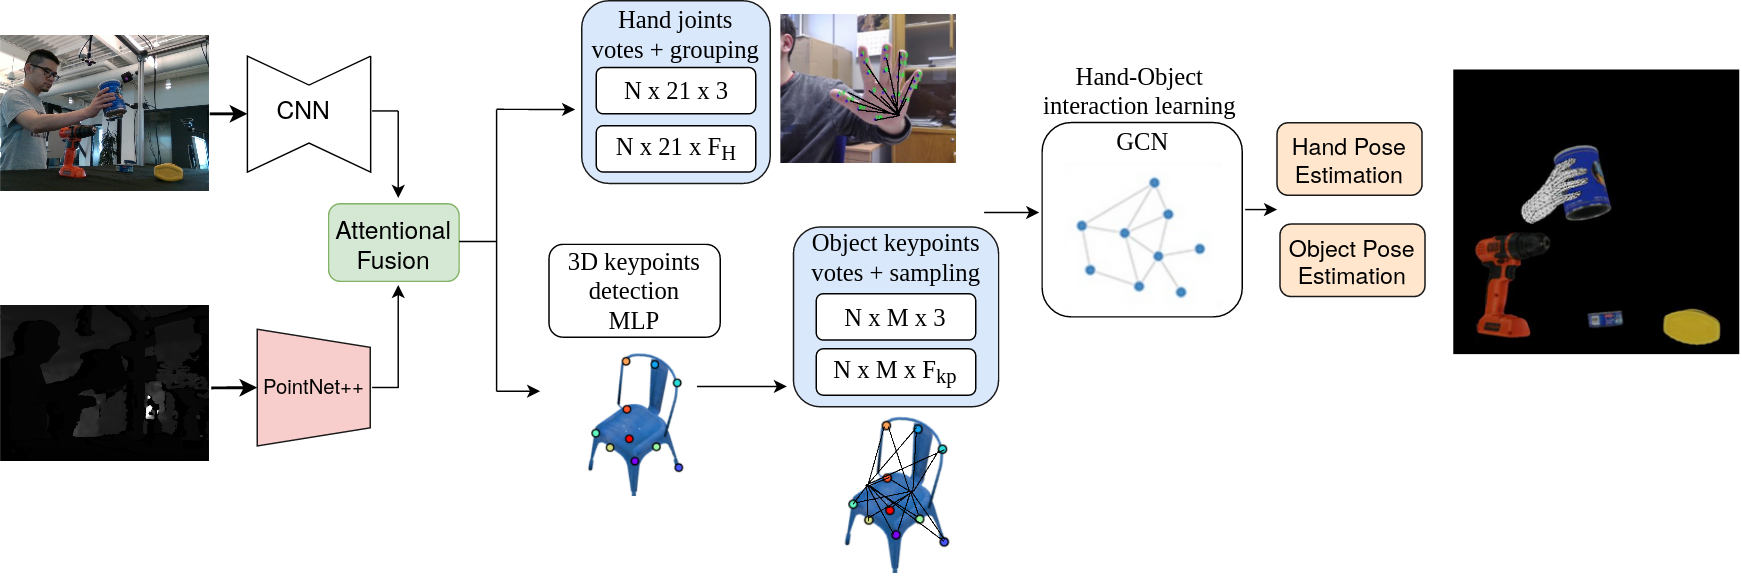
\includegraphics[width=0.95\linewidth]{Figs/Hand-Object_pose.png}
	\caption{\textbf{Overview of our proposal}. Our method takes both color and depth maps as input data. The color features are extracted by a CNN, while the 3D features are calculated by PointNet++ architecture. These two types of features are then fused at a pixel level to obtain the new distinctive features by the adaptive fusion network. This network learns to predict the weight matrix that facilitates beneficial features to eclipse the tedious information. We design a deep Hough voting-based network to vote for 21 MANO hand joints and $M=9$ selected object keypoints. A GCN-based network is deployed to learn the constraints and interdependencies between the hand and object poses to boost the estimation performance.}
	\label{fig:Hand_pose}
\end{figure*}


\subsection{Hand-object pose estimation}
The naive approach for this mission is treating the hand \cite{yang2022dynamic, madadi2017end, deng2017hand3d, oberweger2017deepprior++, iqbal2018hand} and manipulated object \cite{wang2019densefusion, schwarz2015rgb, qi2018frustum, zhou2018voxelnet} separately without considering their interdependence. They underestimate the extraordinary relationship between hand gestures and object shapes. Several approaches overcome this problem by jointly learning the shapes of both hands and objects from RGB images.  \cite{hasson2020leveraging} looks into photometric consistency between neighboring frames to reconstruct hand-object shapes under interactions. \cite{tekin2019h+} handles hand action classification to assist the process of estimating hand-object interactions. \cite{liu2021semi} introduce a semi-supervised learning framework leveraging spatial-temporal consistency to improve estimation performance. However, the absence of depth information makes the process of learning physical constraints and interactions latent. In addition, the transformation from 2D to a 3D world is accurately difficult due to the high degree of nonlinearity. In contrast, some methods solely exploit depth images. \cite{choi2017robust} designs an architecture that firstly predicts hand and object centers and then learns global orientations and hand grasp configurations while interacting with objects. \cite{zhang2021single, goudie20173d} segments 2D hand and object regions from depth images and then optimizes the reconstruction process of interacting motions. This method, however, learns the depth images by a 2D CNN backbone and hence cannot radically observe the geometric information. \cite{oberweger2019generalized} deploys a feedback loop to revise the flawed estimation results using depth images only. RGB-D input, on the other hand, has received relatively less attention due to the puzzle of an effective collaboration of two distinctive input formats still holds a secret. \cite{kyriazis2013physically} focuses on the physical laws of hand actions from RGB-D input to benefit hand-object interaction interpretations. \cite{tsoli2018joint} tracks hands and objects in dealing with a complex scenario in which manipulated objects are deformable. 

\subsection{RGB-D fusion}
With the common of color-depth camera, a wide range of computer vision research such as object segmentation \cite{chen2021global, chen2020bi, park2017rdfnet, zhang2021non} and 6D object detection \cite{wang2019densefusion, tian2020robust, saadi2021optimizing} has been inspired to learn and incorporate color and depth features from RGB-D images. The RGB image and depth image belong to different modalities, so most fusing feature methods are \cite{wang2021brief}: image layer fusion, feature layer fusion, and output layer fusion. While image layer fusion concatenates the input data before feeding to CNNs, feature layer fusion means learning color and depth data in two distinguished architectures but sharing the learning process. Output layer fusion, on the other hand, integrates two feature maps that are separately extracted by two backbone networks. However, fusion RGB-D features for hand-object pose estimation is less attractive because most of the mentioned methods have a mutual weak point which is extracting features from depth maps by 2D CNNs. This makes the 3D spatial feature output latent and oblivious. Motivated by \cite{wang2019densefusion}, we develop a network that not only exports geometric information and geometric constraints by using Pointnet++ \cite{qi2017pointnet++}, but also adaptively and selectively adjusts features at each pixel before fusing to achieve the reliable performance. 

\subsection{Graph convolutional network  for pose estimation}
The power of graph convolutional networks has recently captured the researchers' attention in solving the problem of pose estimation. The network provides the relationship awareness of input data, hence can cope with the problem of a large number of DoF in hand pose estimation. \cite{kong2020sia} allows the network to be spatially aware to boost the 2D hand keypoints prediction. Interm of jointly estimate hand-object pose estimation, \cite{doosti2020hope} develops two graph convolutional network-based architectures for two missions. The first one detects 2D hand joints and 2D object corners, while the second lifts 2D keypoints to 3D coordinates. \cite{almadani2021graph} also designs two steps of firstly predicting 2D hand-object poses. Afterward, this method boosts the performance by gradually providing more information such as the third dimension and mesh vertices to the graph-based network. \cite{tse2022collaborative} proposes attention-guided graph convolution to iteratively share hand and object estimator between two branches for learning the mutual occlusion. This success inspires us to develop a graph-based network for hand-object interaction learning but instead directly feed the 3D features to learn the relationship without the need of lifting 2D information to 3D coordinates, which might cause unpredictable mistakes.

%
\section{Method}
\label{sec:methodology}

\begin{figure*}[t]
	\centering
	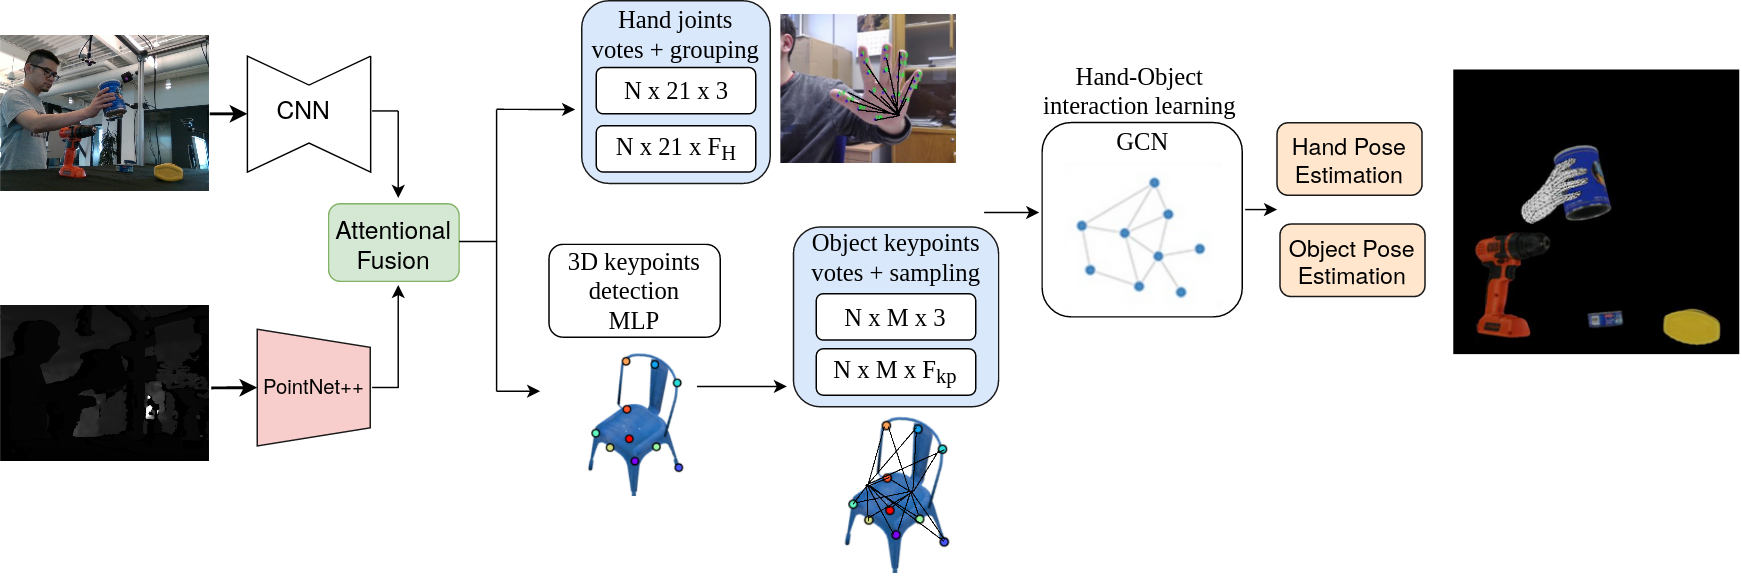
\includegraphics[width=0.95\linewidth]{Figs/Hand-Object_pose.png}
	\caption{Overview of our proposal. Our method takes both color and depth maps as input data. The color features are extracted by a CNN, while the 3D features are calculated by PointNet++ architecture. These two types of features are then fused together at pixel-level to obtain the new distinctive features. The attention mechanism is applied for the such new features to learn the contribution disparity of the context to the hand pose. The votes are computed and then regressed to estimate the MANO parameters.}
	\label{fig:Hand_pose}
\end{figure*}

In Figure \ref{fig:Hand_pose}, we provide an overall pipeline of our method for 3D hand mesh estimation. Our proposed network consists of backbone, Attention, voting and cluster and hand pose Estimation.

\subsection{Attentional Fusion}
\label{sec:attentional_fusion}

\begin{figure}[h!]
	\centering
	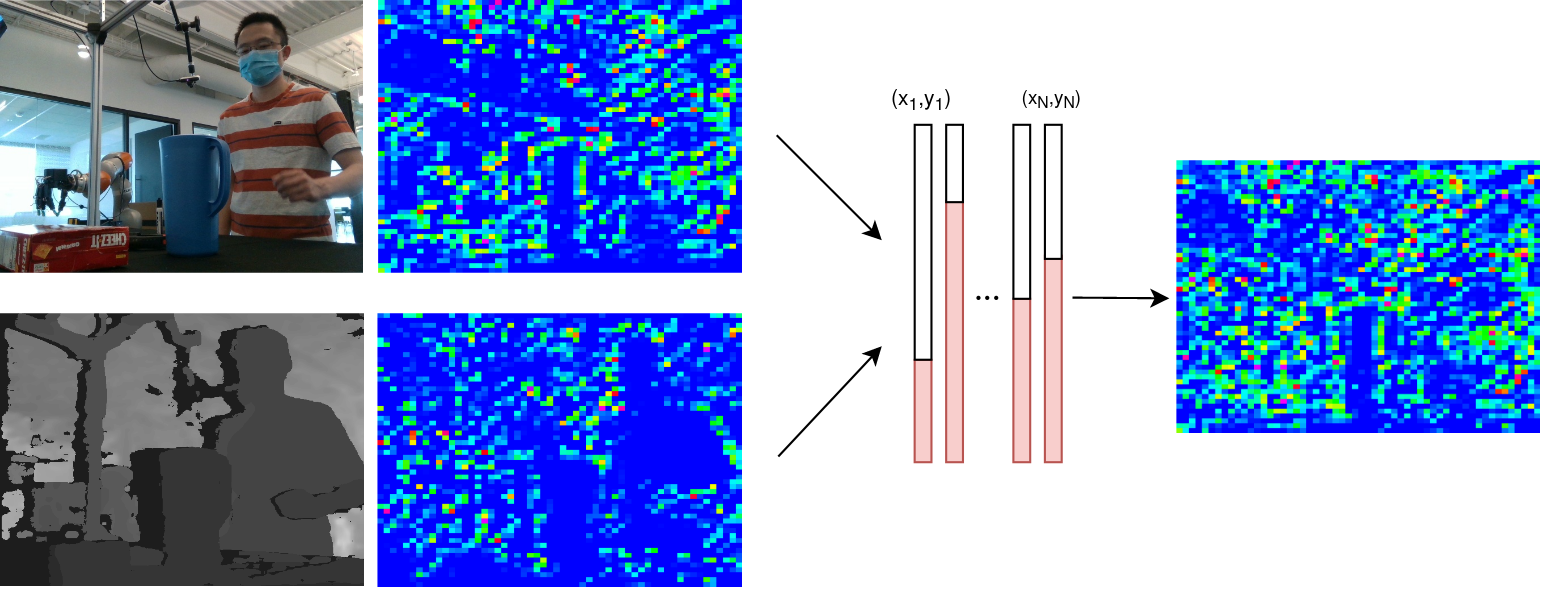
\includegraphics[width=0.9\linewidth]{Figs/Attentional_fusion.png}
	\caption{Attentional fusion.}
	\label{fig:attentional_fusion}
\end{figure}

\textbf{Color feature extraction:} Given a color image $I_{rgb} \in \mathbb{R}^{H \times W \times 3}$, the color features $f_{rgb} = \{ f^{rgb}_i \} ^{H \times W}_{i=1}$ are normally extracted by a CNN architecture. Where $f_{rgb} \in \mathbb{R}^{H \times W \times d_{rgb}}$ and each pixel is mapped into a color feature space $f^{rgb}_i \in \mathbb{R}^{d_{rgb}}$. 

\textbf{Depth feature extraction:} The geometric features, on the other hand, are extracted by converting depth maps to point cloud and then feeding into PointNet \cite{qi2017pointnet}. In our work, differing from the original work, we conduct PointNet++ \cite{qi2017pointnet++}, an upgraded version, to replace the original backbone. Given a depth map $I_d \in \mathbb{R}^{H \times W \times 1}$, the point cloud features $f_{geo} = \{f^{geo}_i\}^{H \times W}_{i=1}$.

\textbf{Feature Embedding:} Numerous methods integrate color features and geometric features into each other without considering the fact that the distribution of informative features at each position is not equal. Our proposal module termed attentional fusion aims to learn the contributing ability of each pixel feature for effectively fusing procedure. To obtain this, we add learnable weight matrix to either widen or inhibit the pixel feature across the whole image. Where $A$ and $B$ are learnable hyper-parameters. $f^{fusion} \in \mathbb{R}^{H \times W \times (d_{rgb} + d_{geo})}$.

\begin{equation}
	f^{fusion} = A \times f^{rgb} \oplus B \times f^{geo} \
\end{equation}

\subsection{Hand and Object Voting}
\label{sec:voting}
\textbf{Hand joints voting:} As shown in \ref{fig:Hand_pose}, the discriminative features with rich information after fusing procedure are used to regress hand joints. Conventional voting methods approaching object pose estimation including hand poses usually vote for the hand center. Whereas, our method computes votes for hand joints points due to the fact that hand joints can reflect the hand gestures, which is crucial for hand pose estimation under interaction. The hand joints convey information about the hand shape itself but also 3D object shape. Therefore, such hand joints are neccessary for hand-object interaction learning. We adopt the MANO hand mesh model \cite{romero2022embodied} with 21 hand keypoints $J$ consisting of 16 original hand joints and 5 hand vertices. 

Given the point cloud $\{ p_i \}^{N_{\mathcal{H}}}_{i=1}$ and 21 MANO hand keypoints $\{ Hkp_j \}^{21}_{j=1}$ belong to the same hand $\mathcal{H}$. We denote $p_i = [x_i, f^{fusion}_i]$ with $x_i$ the 3D coordinate and $f^{fusion}_i$ the attentionally fused feature. Similarly, we denote $Hkp_j = [x^{Hkp}_j]$ with $x^{Hkp}_j$ the 3D coordinate of the hand keypoints. We compute the translation offset $\{ {\Delta_{Hkp}}^j_i \}^{21}_{j=1}$ for each point, where ${\Delta_{Hkp}}^j_i$ denotes the translation offset from the $i_{th}$ point to the $j_{th}$ hand keypoint. Thevoted keypoint can be computed as $vHkp^j_i = x_i + {\Delta_{Hkp}}^j_i$. We define the loss for hand keypoints learning as below:
%%%%%%%%%%%%%
\begin{equation}
	\mathcal{L}_{Hkp} = \frac{1}{N_{\mathcal{H}}} \sum_{i=1}^{N_{\mathcal{H}}} \sum_{j=1}^{21} \|{\Delta_{Hkp}}^j_i - {\Delta_{Hkp}}^{j*}_i \|_H \cdot \mathds{1}(p_i \in \mathcal{H}) \
	\label{eq:loss_handjoints}
\end{equation}
%%%%%%%%%%%%%
where ${\Delta_{Hkp}}^{j*}_i$ is the ground truth translation offset, $N_{\mathcal{H}}$ is the total of number of points belonging to a hand $\mathcal{H}$. $\| \cdot \|_H$ is the Huber norm. The binary function $\mathds{1}(\cdot)$ equals to 1 when point $p_i$ belongs to a hand $\mathcal{H}$, and 0 otherwise.

\textbf{Object keypoints Selection:} The 3D keypoints are selected from 3D object models. Normally, eight corners of 3D bouding box are used to represent the object. However, the corner points are actually far away from point on object, leading to the difficulty to infer the physical constrains while interacting with the hand. Therefore, we instead select keypoints on the object surfaces that provide ease to learn the hand-object interaction. We use the farthest point sampling (FPS) algorithm to collect the keypoints of objects by initilizing a object mesh center point as the first keypoint and the searching the others by FPS until obtain $M$ keypoints. 

\textbf{Object keypoints voting:} In terms of learning the object presence, the attentionally fused features is fed into a module to predict 3D keypoints for each object. Concretely, given a set of points $\{ p_i \}^{N_{\mathcal{O}}}_{i=1}$ and $M$ selected object keypoints $\{ Okp_j \}^{M}_{j=1}$ belong to the same object $\mathcal{O}$. We denote $Okp_j = [x^{Okp}_j]$ with $x^{Okp}_j$ the 3D coordinate of the object keypoints. The translation offset from the $i_th$ point to the $j_th$ object keypoints is denoted as ${\Delta_{Okp}}^j_i$. Hence, for each point we generate translation offset $\{ {\Delta_{Hkp}}^j_i \}^{M}_{j=1}$. The voted object keypoint can be computed as $vOkp^j_i = x_i + {\Delta_{Okp}}^j_i$. We define the loss function as below:
%%%%%%%%%%%%%%%%%%%%%%%%%%%%%%
\begin{equation}
	\mathcal{L}_{Okp} = \frac{1}{N_{\mathcal{O}}} \sum_{i=1}^{N_{\mathcal{O}}} \sum_{j=1}^{M} \|{\Delta_{Okp}}^j_i - {\Delta_{Okp}}^{j*}_i \|_H \cdot \mathds{1}(p_i \in \mathcal{O}) \
	\label{eq:loss_objectpoints}
\end{equation}
%%%%%%%%%%%%%%%%%%%%%%%%%%%%%%%
where ${\Delta_{Okp}}^{j*}_i$ is the ground truth translation offset, $N_{\mathcal{O}}$ is the total of number of points belonging to an object $\mathcal{O}$. $\| \cdot \|_H$ is the Huber norm. The binary function $\mathds{1}(\cdot)$ equals to 1 when point $p_i$ belongs to an object $\mathcal{O}$, and 0 otherwise.

\subsection{Hand and Object Poses Estimation}
\label{sec:interaction}
\begin{figure}[h!]
	\centering
	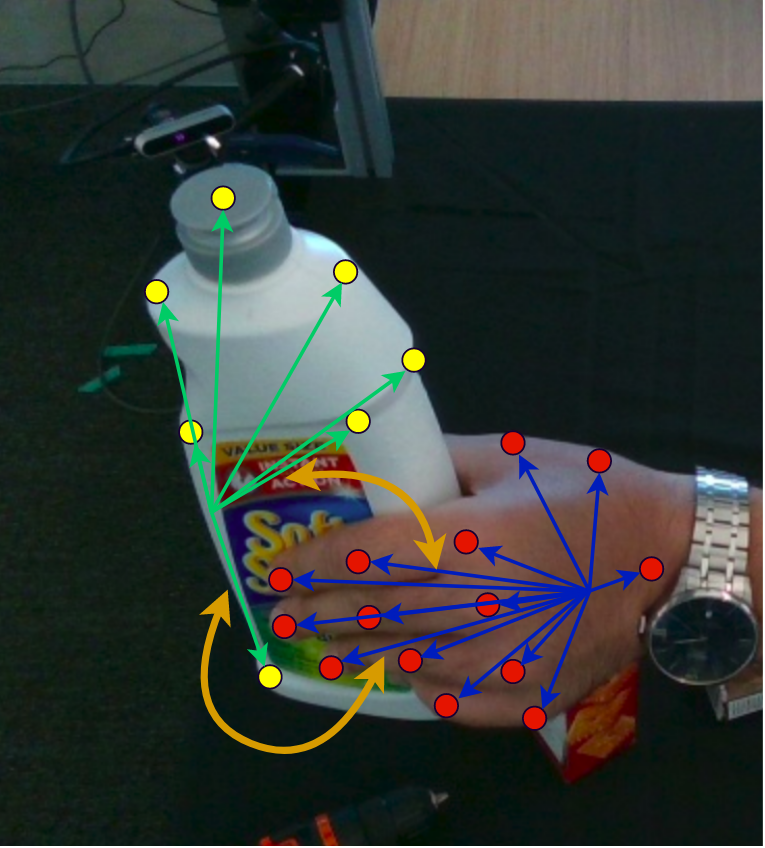
\includegraphics[width=0.6\linewidth]{Figs/Hand-object.png}
	\caption{Illustration of the interaction learning between votes for hand keypoints and votes for object keypoints. The red points denote hand keypoints, while the yellow ones denote object keypoints. The blue and green vectors represent hand keypoints and object keypoints votes, respectively.}
\end{figure}
\textbf{Hand-object interaction learning:} To estimate the hand and object shapes under interactions, voting vectors should be aware of their global neighborhood. Esecially, the object keypoints in a vicinity are intuitively benificial for the predicting hand keypoints and vice cersa. We adopt a graph convolutional network (GCN) for interaction learning procedure. Each node of the graph is defined by the proposal position $y_i$ associated with proposal feature $g_i$. In particular, the proposal position is either hand keypoint $(y_i = vHkp^j_i)$ or object keypoint $(y_i = vOkp^j_i)$ and the associated proposal feature $g_i=f^{fusion}_i$. An edge between two nodes is determined by checking the condition of Euclidean distance between them. If the distance between two neighboring positions $(d_{y_i, y_j} < \delta)$, the edge-feature is defined as:
%%%%%%%%%%%%%%%%%%
\begin{equation}
	e_{ij} = \mathit{h}([y_i,g_i],[y_j, g_j]-[y_j,g_j]) \
	\label{eq:edge_feature}
\end{equation}
%%%%%%%%%%%%%%%%%%%%%%%%%%
where $\mathcal{h}$ is a non-linear fuction. Obtain refined proposal features from intial fusion featues. 

\textbf{Hand and Object pose regression:} we adpot the MANO hand mesh model defined a manifold triangle mesh $M = (V,F)$ to estimate the final hand pose. $V = \{ v_i \in \mathbb{R}^3 \} \| 1 \leq i \leq n$ is a set of $n=778$ vertices and $F$ is a set of faces. They are parameterized by the MANO parameters $(\theta \in \mathbb{R}^{51}, \beta \in \mathbb{R}^{10})$. We use multi-layer perceptron (MLP) to regress the parameters $(\theta, \beta)$. We define the loss fuction for hand pose regression as below, where the hand keypoints loss $\mathcal{L}_{Hkp}$ as equation \ref{eq:loss_handjoints}.
%%%%%%%%%%%%%%%%%%%%%%%%%%%%%%%%%%%
\begin{equation}
	\mathcal{L}_{handpose} = \mathcal{L}_{Hkp} + \mathcal{L}_V + \mathcal{L}_{\theta} + \mathcal{L}_{\beta} \
	\label{eq:loss_handpose}
\end{equation}
%%%%%%%%%%%%%%%%%%%%%%%%%%%%%%%%%%%

In terms of regressing the object pose, we embrace the procedure that maps 6D vectors in representation space produced by the network into the original rotation space and minimizes the differencies between the output and the ground-truth rotation matrices. The rigid transformation consists of a rotation $R \in SO(3)$ and a translation $t \in \mathbb{R}^3$. We define the loss function as below:
%%%%%%%%%%%%%%%%%%%%%%%%%%%%%%%%%%%
\begin{equation}
	\mathcal{L}_{objectpose} = \mathcal{L}_{Okp} + \mathcal{L}_t + \mathcal{L}_R	\
	\label{eq:loss_handpose}
\end{equation}
%%%%%%%%%%%%%%%%%%%%%%%%%%%%%%%%%%%
where the loss for object keypoints voting $\mathcal{L}_{Okp}$ is defined as equation \ref{eq:loss_objectpoints}, $\mathcal{L}_t$ is the translation loss. The above rotation loss $\mathcal{L}_R$ is appropriate to asymmetric objects. The rotation metric for symmetric objects is diverse, therefore, given the estimated rotation $\overline{R}$ and translation $\overline{t}$ and the ground-truth $(R^*, t^*)$. The rotation loss redefined as below:
%%%%%%%%%%%%%%%%%%%%%%%%%%%%%%%%%%%
\begin{equation}
	\mathcal{L}_R = \frac{1}{m} \sum_{x_1 \in \mathcal{M}} \| \min\limits_{x_2 \in \mathcal{M}} (\overline{R}x + \overline{t} - R^*x - t^*) \| \
\end{equation}
%%%%%%%%%%%%%%%%%%%%%%%%%%%%%%%%%%%
where $\mathcal{M}$ denotes the 3D object models and $m$ is the number of points.

Finally, the loss function for hand-object pose estimation under interaction summarized as below:
\begin{equation}
	\mathcal{L}_{hand-object} = \mathcal{L}_{handpose} + \mathcal{L}_{objectpose} \
	\label{eq:hand-object}
\end{equation}



%
\section{Evaluation}
\label{sec:Eval
}
%
{\small
\bibliographystyle{ieee_fullname}
\bibliography{egbib}
}

\end{document}
